\documentclass[10pt,handout,english]{beamer}
\usetheme{Berlin}
\usecolortheme{seahorse}
\usepackage{amsmath}

\usepackage{listings}
\definecolor{mymauve}{rgb}{0.58,0,0.82}
\definecolor{mygreen}{rgb}{0,0.6,0}


\usepackage{graphicx} %%For loading image files
\graphicspath{ {images/} } %folder-location for images

\title[] % (optional, only for long titles)
{Python API for Mobile Robot Control}
\subtitle{Final Presentation}
\author[AE-663 Course Project 2016-17] % (optional, for multiple authors)
{Parin Chheda (153076005) \\ Saurav Shandilya (153076004) \\ Group-10 }
\institute [Indian Institute of Technology Bombay]% (optional)
{
  
}
\date[\today] % (optional)
{Prof. Prabhu Ramachandran \\ Prof. Madhu Belur \\ Prof. Kumar Appaiah}
%\subject{Computer Science}

\begin{document} 
	\lstset{language=C,commentstyle=\color{mygreen},showspaces=true,   
		showstringspaces=false, basicstyle=\footnotesize,  
		breakatwhitespace=false,keepspaces=true,            breaklines=true,stepnumber=1,showspaces=false} 
\frame{\titlepage}

\begin{frame}{Objective}
\begin{enumerate}
	\item A Python API to control the different peripherals of the ${\mu}$controller
	\item Provide the user with a option of register level access of the ${\mu}$controller
	\item Allow the user to design an application without learning a new language and thoroughly knowing the architecture of the controller.
\end{enumerate}
\end{frame}

\begin{frame}{Task Accomplished}

\begin{enumerate}
	\item enter details

\end{enumerate}

\end{frame}

\begin{frame}{Git Commit Graphs}
%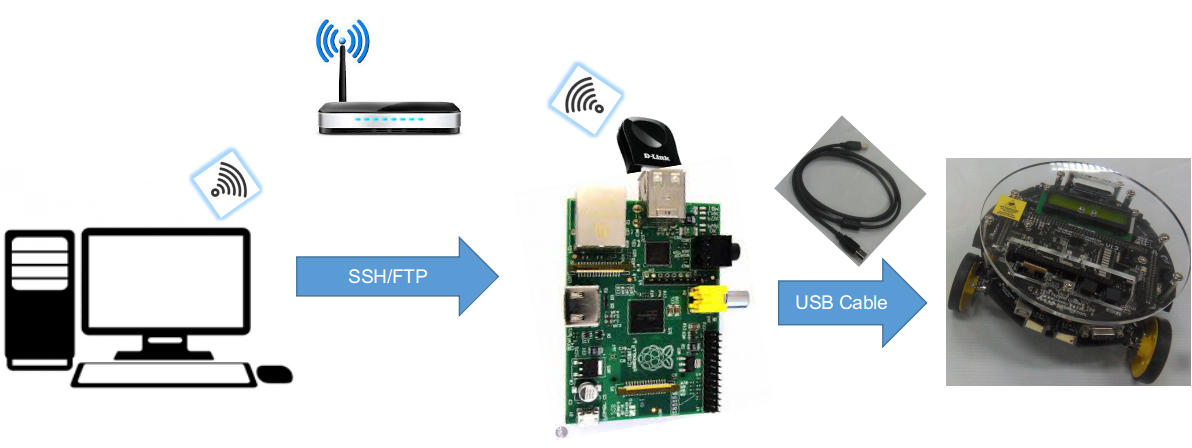
\includegraphics[scale = 0.35]{system_diagram}
how many commts.
  Git commit history, timeline, graphs, put in slide

\end{frame}

\begin{frame}{Code Test Coverage}
	testsuite running in verbose mode
	    Show coverage in slides.
	    nose, pytest,
\end{frame}

\begin{frame}{Automation}
Travis-ci - 
Coverall

make file
    setup
    setup.py yes/no:

\end{frame}

\begin{frame}{Documentation}
Read the docs yes/no.
    shpinx screenshot.
    Documentation:
    docstrings?

\end{frame}


\begin{frame}{Pep8 Compilance}
	Pep8 followed?
    What is their API.
    How should a user use?
\end{frame}

\begin{frame}{Challenges Faced}
	\begin{itemize}
		\item API implementation
			\begin{itemize}
				\item Configuring serial 
			\end{itemize}
	\end{itemize}
	
\end{frame}


\end{document}
